% ---------------------------------------------------
% ----- Chapters of the template
% ----- for Bachelor-, Master thesis and class papers
% ---------------------------------------------------
%  Created by C. Müller-Birn on 2012-08-17, CC-BY-SA 3.0.
%  Freie Universität Berlin, Institute of Computer Science, Human Centered Computing. 
%
% TODO remove 2 - to use auto numbering
\chapter{4 - User research and analysis}
\label{chap:chapters}


% Due to the limited size of the user group, the goal was not to gain <TODO> with high diversity of their demographics, but to have information saturation from fewer but more valuable insights into peolpe with diffrent workflows.

To avoid the common problem in software development where products are built based on the ideas of individual stakeholders who may not even use the product,
instead of relying on meaningful user input,
I applied various methods of user research commonly used in Human-Computer Interaction (HCI) and evaluated their effectiveness in the context described earlier.

A starting point for qualitative user research is to define the goals through the help of the SMART Criteria <TODO cite>.

For these criterias, I defined the overall goal as following:

\begin{itemize}
  \item \textbf{specfic} - improve the workflow of users modifying dynamic resources
  \item \textbf{measurable} - interviews after testing period, concerning working speed and confidence when editing resources, user tracking
  \item \textbf{assignable} - research implementation will mostly be conducted by me, with input from CTO \& product owner, connection to external users through customer service team
  \item \textbf{realistic} - new software platform which reacts quicker, prvides more safety regarding errors and is scalable and extensible in the future. Limiting factors are time (as I only have three months for the first phase, including writinh this thesis)
  \item \textbf{time-related} - the new software should have at least the same feature set and be usable by company-internal users until the end of 2022
\end{itemize}
\section{Identifying and categorizing users and user groups}

In order to effectively design and implement the UI editor, it is crucial to understand the needs and preferences of the various users and user groups who will be using the tool.
Therefore, the first step in the user research process was to identify and categorize the different users and user groups who will be using the editor.
This included both internal and external users, as well as users with different levels of experience and expertise. By understanding the characteristics and needs of each user group, we can ensure that the UI editor is tailored to their specific requirements and can be used effectively by all users.
\\
As explained earlier, because we had a preceeding, less powerfull tool to edit the resources, which was used mostly by company-internal developers and managers,
but also available to some external customers. As a first step, I collected a list of mail adresses that accessed the tool by looking at the logs, and wrote a mail to our developers who would be interested in working with me for both design phase and later as alpha and -beta testers.

Then, I derived the follwoing commomn factors from the users, most of which I personally know, which made the communication and categorization a lot easier.

\begin{itemize}
  \item \textbf{quantitative usage} There were users who relied on the tools for most of their work, while others like the external customers accessed the tool a few times a year.
  \item \textbf{common tasks} I <grob> categorized the common tasks into three groups:
    \subitem \textbf{Heavy configuration} Mostly internal devs used the tools to build new apps and websites from scratch (or derived from exisiting apps), making many modifications, from structural changes to the seperate views, menus, data sources and more, over styling and translating messages to diffrent languages.
    \subitem \textbf{Moderate configuration} Project devs and customer support people copy resources from existing apps and adapt them for new brands, which often includes changing colors and logos, adapting texts or switching authentification flows.
    \subitem \textbf{Small changes} External customers often only use the tools to exchange some ads, translations or logos, which affects a small set of files.
  \item \textbf{expertise} <kann man bei schlechter software gut erkennen, leute mit viel erfahrung checken sachen, aber ist für neue nicht intutitiv>
\end{itemize}

% ... more

\section{Process and vizualize the outcomes of the initial user research phase}

\subsection{2x2 Opportunity Matrix}

This two-dimensional vizualization of a set of proposed features prooved helpful when prioritizing tasks with other stakeholders,
as it shows the (approximated) cost of implementation as well as the value the feature can have for users.

The matrix I used is a slightly modified adaption from \cite[p. 181]{LearnHCI:2020ys}, replaced the term ''idea originality'' on the x-axis with ''Value''.

\begin{figure}[ht]
	\centering
  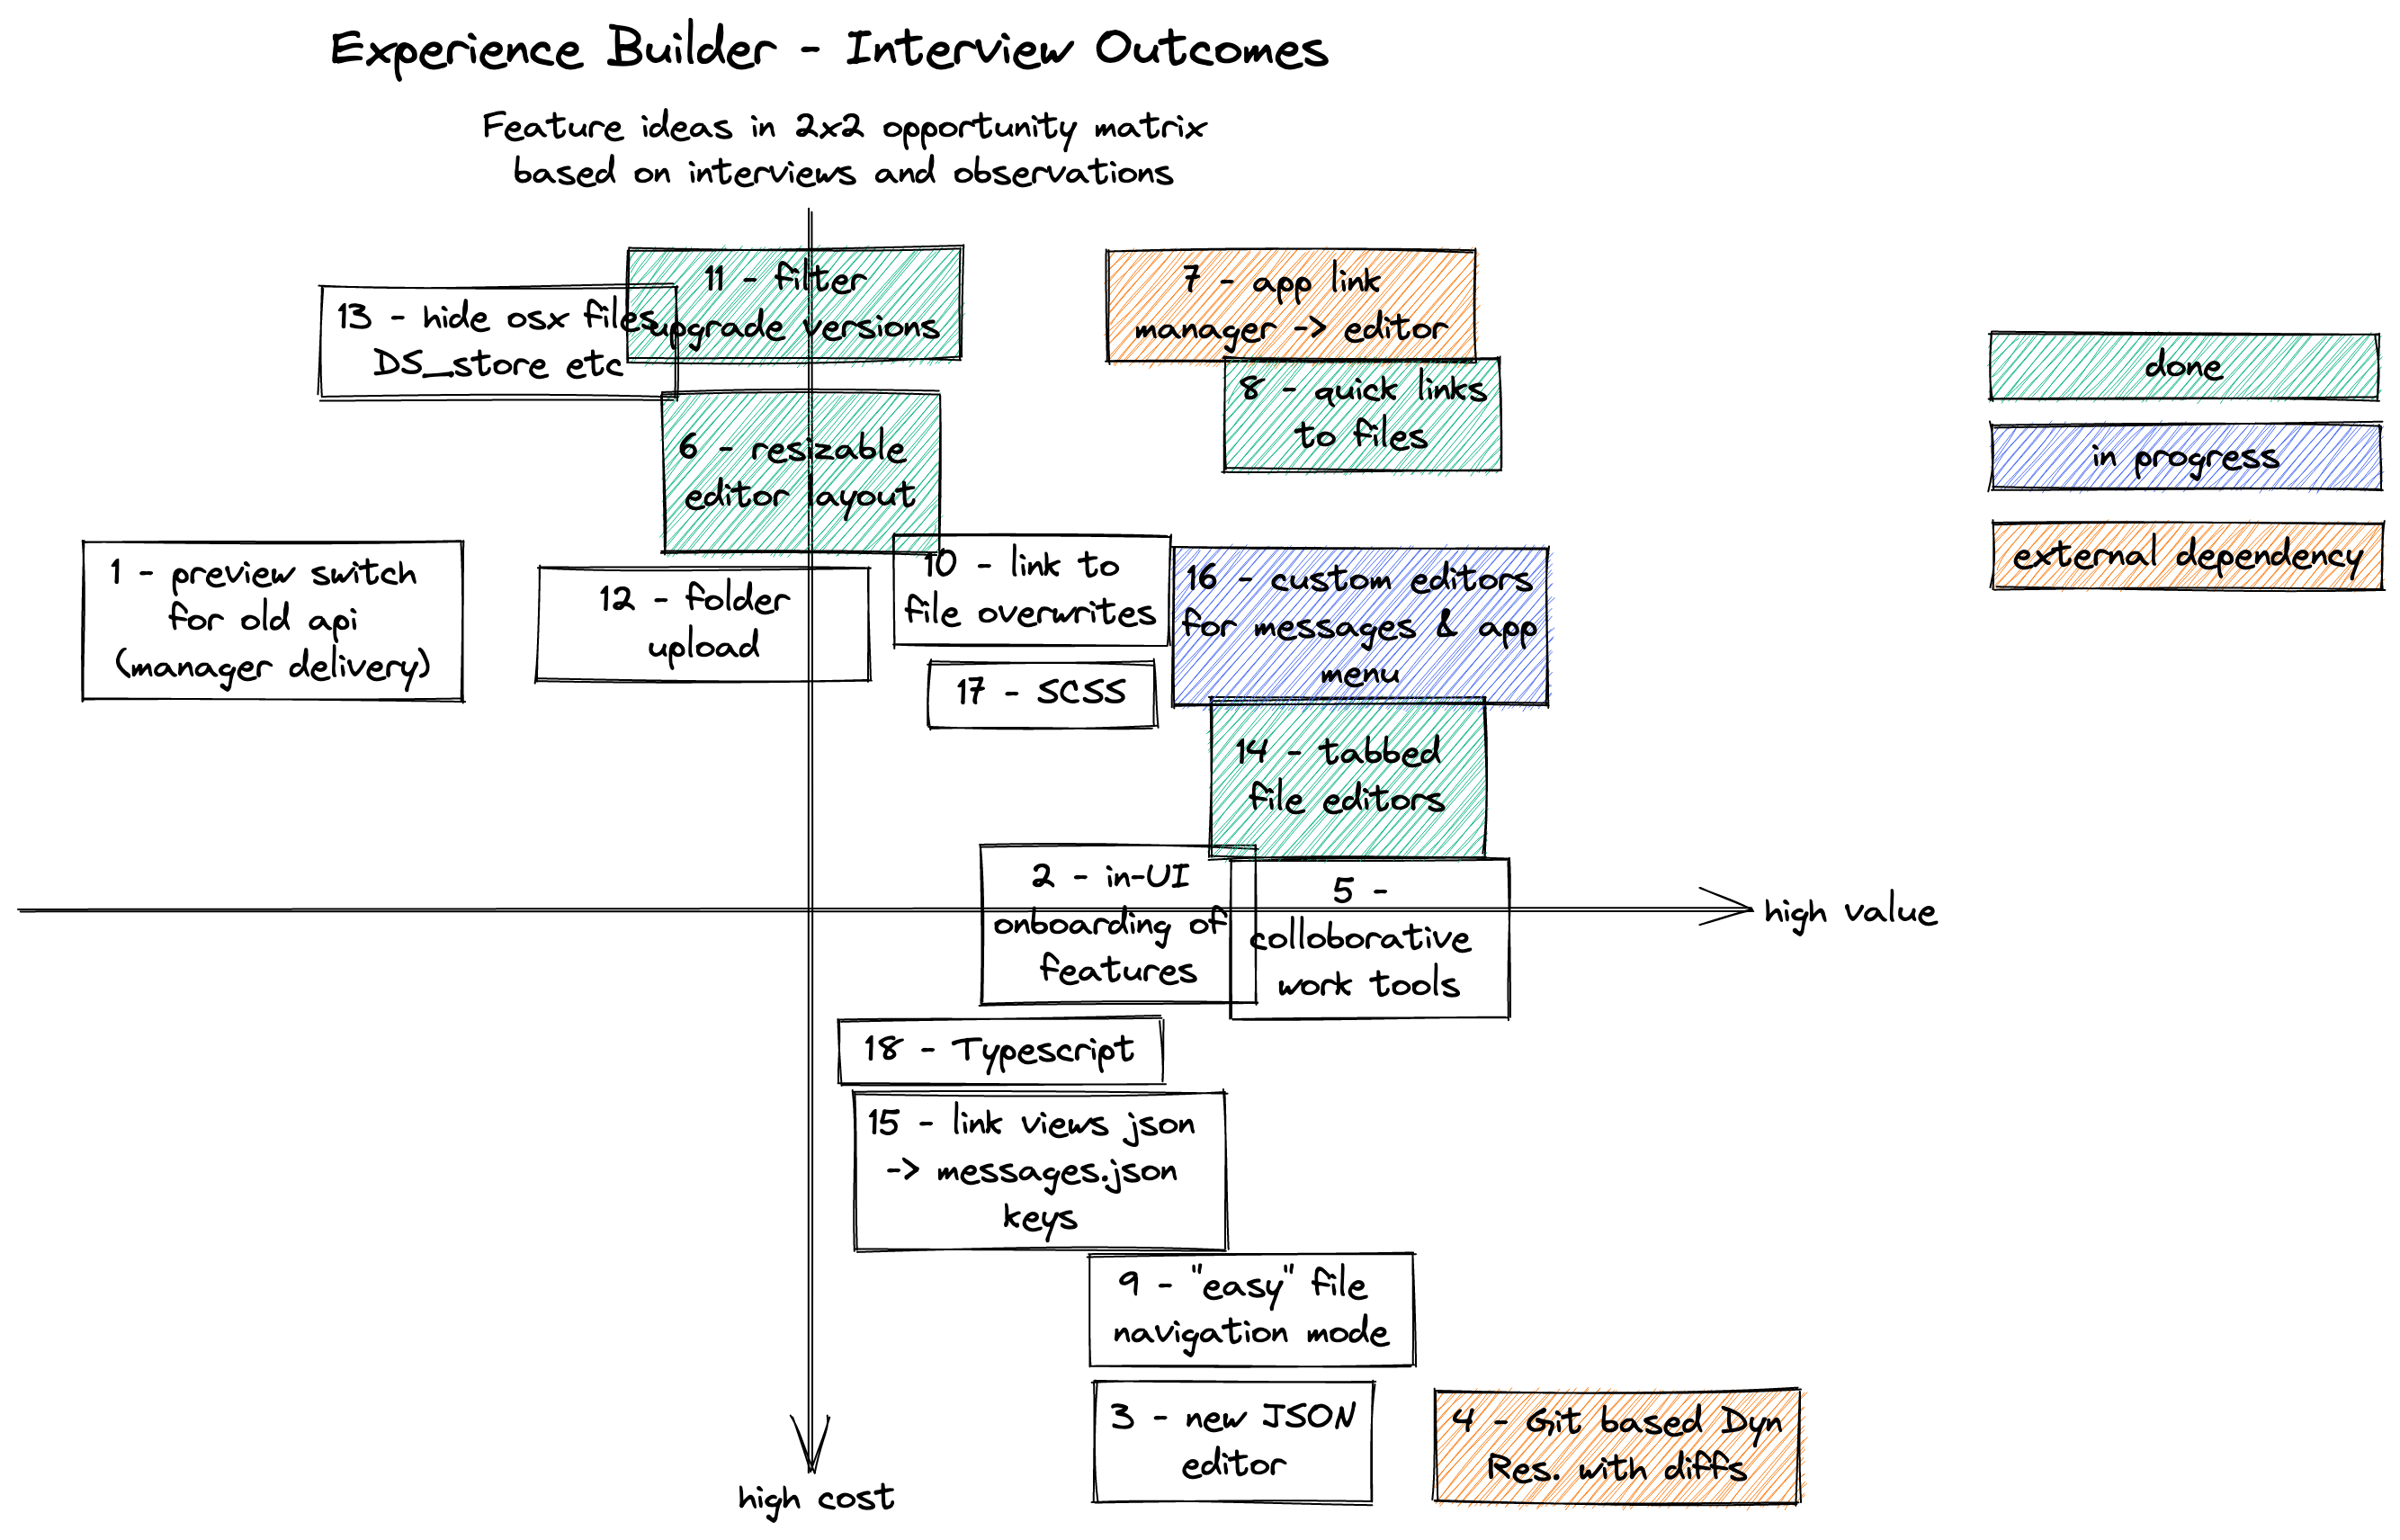
\includegraphics[width=\textwidth]{pics/feature_cost_matrix.excalidraw.png}
	\caption{2x2 Opportunity Matrix during the early phases of development}
	\label{fig:opportunitymatrix}
\end{figure}
